\centerline{\bf \Huge 10 класс}

\problem{1}
Каждую грань кубика разбили на четыре одинаковых квадрата, а затем раскрасили эти квадраты в несколько цветов так, что квадраты, имеющие общую сторону, оказались окрашенными в различные цвета. Какое наибольшее количество квадратов одного цвета могло получиться?

\textit{Решение.} 
Докажем от противного, что одноцветных квадратов меньше 9. Пусть возможно получить 9 или больше одноцветных квадратов. Каждый квадрат прилегает к одной вершине куба. У куба 8 вершин, поэтому хотя бы два из наших одноцветных квадратов примыкают к одной и той же вершине куба. Но примыкающие к одной вершине квадраты имеют общую сторону, противоречие.

Пример развертки для 8 квадратов приведен на картинке. Серые квадраты одноцветные, белые можно покрасить, например, в 16 различных цветов.

\begin{figure}[h]
    \centering
    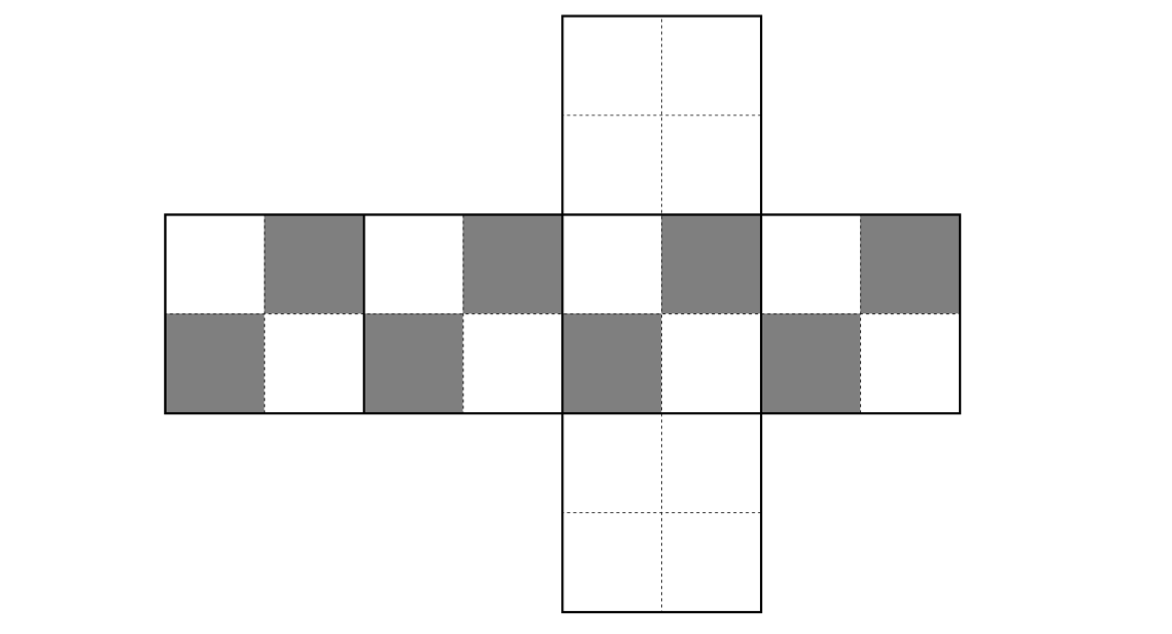
\includegraphics[width=0.5\linewidth]{Эльзята/Contest_9_1.png}
    \caption{Развертка куба}
    \label{fig:placeholder}
\end{figure}

\problem{2}
Внутри параллелограмма $A B C D$ выбрана точка $E$ так, что $A E=D E$ и $\angle A B E=90^{\circ}$. Точка $M$ - середина отрезка $B C$. Найдите угол $D M E$.

\textit{Решение.}
Обозначим через $N$ середину отрезка $A D$. Поскольку треугольник $A E D$ равнобедренный, его медиана $E N$ является высотой, то есть $E N \perp A D$. Значит, $N E \perp B C$ (см. рис. 2).

Поскольку $A D \| B C$ и $B M=M C=A N=N D=A D / 2$, четырёхугольники $A B M N$ и $B M D N$ - параллелограммы, откуда $A B \| M N$ и $B N \| D M$. Так как $\angle A B E=90^{\circ}$ и $A B \| M N$, получаем $B E \perp M N$. Таким образом, $E$-точка пересечения высот треугольника $B M N$, откуда $M E \perp B N$. Наконец, из $B N \| D M$, получаем $M E \perp D M$, то есть $\angle D M E=90^{\circ}$.

\begin{figure}[h]
    \centering
    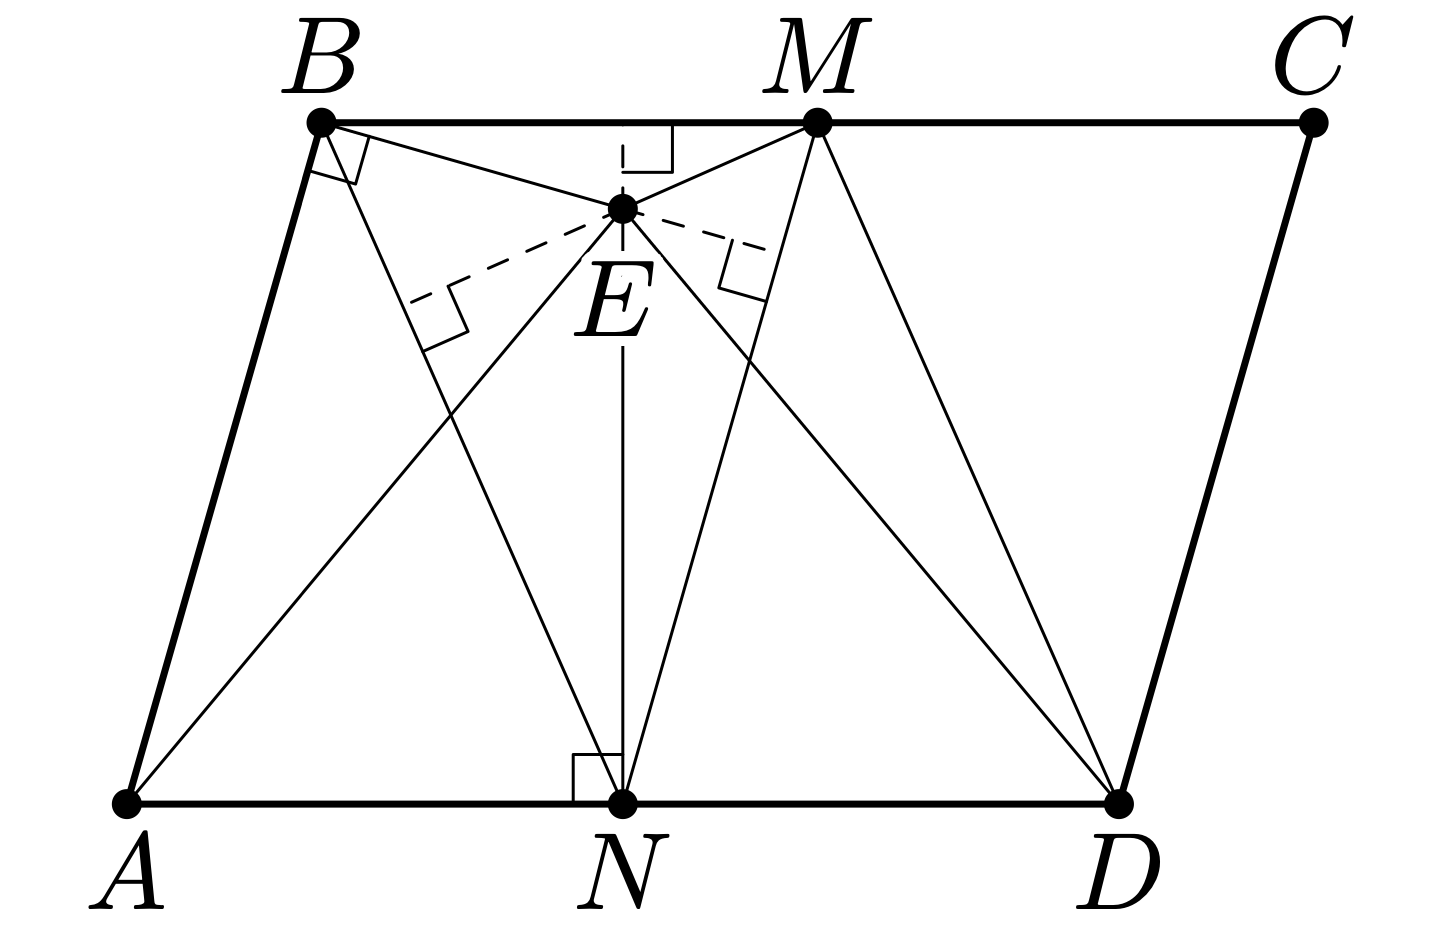
\includegraphics[width=0.5\linewidth]{Эльзята/Contest_9_2.png}
    \caption{}
    \label{fig:placeholder}
\end{figure}

\problem{3}
Множество состоит из целых чисел, причем в нем есть и положительные, и отрицательные числа. Если числа $a$ и $b$ содержатся в множестве, то в нём также содержатся числа $2 a$ и $a+b$. Докажите, что это множество содержит разность любых двух своих элементов.

\textit{Решение.} Назовем наше множество $A$. Пусть $m_{+}$- наименьшее положительное число из $A$, пусть $m_{-}$- наибольшее отрицательное число из $A$. (Оба числа существуют по условию).

Заметим, что $m_{+}=-m_{-}$. Действительно, если $m_{+}>-m_{-}$, то $0<m_{+}+m_{-}<m_{+}$, что противоречит минимальности $m_{+}$. Случай $m_{+}<-m_{-}$аналогично невозможен.

$A=\left\{k m_{+} \mid k \in \mathbb{Z}\right\}$. Действительно, $1 \cdot m_{+} \in A$ и если $k m_{+} \in A$, то $(k+1) m_{+}=k m_{+}+m_{+} \in A$ и $(k-1) m_{+}=k m_{+}+m_{-} \in A$, то есть $A \supset\left\{k m_{+} \mid k \in\right. \mathbb{Z}\}$. Пусть теперь $a \in A, a=k m_{+}+r, 0 \leqslant r<m_{+}$. Тогда $r=a+\left(-k m_{+}\right) \in A$ (мы уже доказали, что $-k m_{+} \in A$ ). Следовательно, $r=0$, так как иначе получаем противоречие с минимальностью $m_{+}$. Поэтому $A=\left\{k m_{+} \mid k \in \mathbb{Z}\right\}$.
Остается тривиальная проверка. Пусть $a_1 \in A, a_2 \in A$. Тогда $a_1=k_1 m_{+}, a_2=k_2 m_{+}$ и $a_1-a_2=\left(k_1-k_2\right) m_{+} \in A$.


\problem{4}
$a, b, c$-стороны треугольника с периметром 1. Докажите неравенство

$$
\frac{1+a}{1-2 a}+\frac{1+b}{1-2 b}+\frac{1+c}{1-2 c} \geqslant 12 .
$$

\textit{Решение.} Перепишем неравенство в виде

$$
\frac{2 a+b+c}{-a+b+c}+\frac{a+2 b+c}{a-b+c}+\frac{a+b+2 c}{a+b-c} \geqslant 12 .
$$


Приведем выражение к общему знаменателю; домножим на знаменатель обе части неравенства. Это можно сделать, так как по неравенству треугольника все знаменатели положительные. После упрощений получаем $T_{3,0,0}+T_{1,1,1} \geqslant 2 T_{2,1,0}$. Это верно по неравенству Шура.
 
\problem{5}
Дана таблица $100 \times 100$. Для любого $k(1 \leqslant k \leqslant 100)$, в $k$-й строке таблицы записаны числа $1,2, \ldots, k$ в возрастающем порядке слева направо, но не обязательно в последовательных клетках; остальные $100-k$ клеток заполнены нулями. Докажите, что найдутся два столбца, сумма чисел в одном из которых хотя бы в 19 раз превосходит сумму чисел в другом.

Решение. Заметим, что сумма чисел в первом столбце не превосходит 100. Докажем, что найдется столбец с суммой чисел $\geqslant 1900$.

Предположим противное.
Посчитаем сумму чисел во всей таблице.

$$
\sum_{i=1}^{100} \frac{i(i+1)}{2}=\frac{100(100+1)(2 \cdot 100+1)}{6 \cdot 2}+\frac{100(100+1)}{2 \cdot 2}=171700 .
$$


Назовем $R$ прямоугольник, образованный первыми 19 столбцами таблицы. Оценим сумму чисел в $R$. Пусть $S_i$ - сумма чисел в $i$-й строке $R$. Тогда:

$$
\begin{aligned}
& S_1 \leqslant 1 ; \\
& S_2 \leqslant 1+2 ; \\
& S_3 \leqslant 1+2+3 ; \\
& \ldots \\
& S_{18} \leqslant 1+\ldots+18 ; \\
& S_{19} \leqslant 1+\ldots+19 ; \\
& S_{20} \leqslant 1+\ldots+19 ; \\
& \ldots \\
& S_{100} \leqslant 1+\ldots+19 .
\end{aligned}
$$


Сложим эти неравенства.

$$
\begin{gathered}
S_{19}+S_{20}+\ldots+S_{100} \leqslant 190 \cdot 82=15580 ; \\
S_1+\ldots+S_{18} \leqslant \sum_{i=1}^{19} i(19-i)=19 \sum_{i=1}^{19} i-\sum_{i=1}^{19} i^2=19 \cdot 190-\frac{19 \cdot 20 \cdot 39}{6}=1140 .
\end{gathered}
$$


По предположению сумма чисел в каждом столбце, не вошедшем в $R$, меньше 1900 . Поэтому общая сумма чисел в таблице меньше чем $15580+1140+81 \cdot 1900= 170620<171700$. Противоречие.